\documentclass[12pt,a4paper]{article}
\usepackage[utf8]{inputenc}
\usepackage{graphicx}
\usepackage{geometry}
\usepackage{enumitem}
\usepackage{titlesec}
\usepackage{hyperref}

\geometry{margin=2.5cm}

\title{Enrolment Trend Analysis}
\date{}

\begin{document}

\maketitle

\section*{1. Monthly Distribution of Students}

As shown in Figure~\ref{fig:monthly-students}, the highest enrolment occurred in July (42 students) and November (41 students). March and June had the lowest enrolment, with only 17 students each. These variations may reflect seasonal effects such as holidays, exams, or changes in marketing efforts.

\begin{figure}[h!]
    \centering
    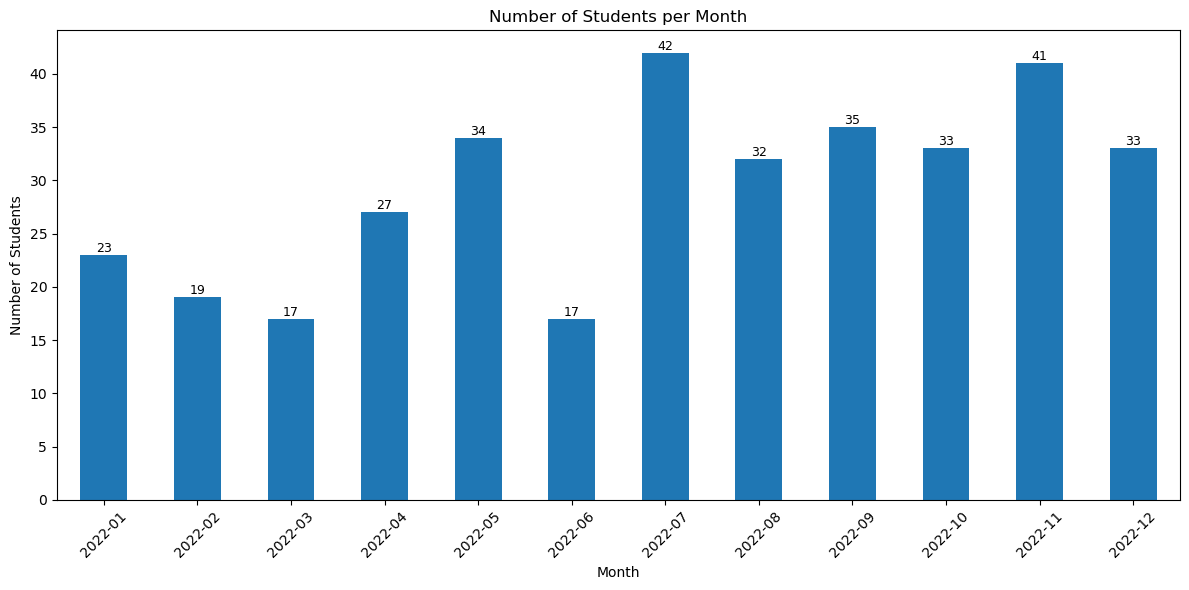
\includegraphics[width=0.9\textwidth]{Number of Students per Month.png}
    \caption{Number of Students per Month}
    \label{fig:monthly-students}
\end{figure}

\section*{2. Seasonal Distribution of Students}

Figure~\ref{fig:seasonal-students} shows the distribution of students by season. Summer (109 students) and Autumn (107 students) had the highest share of enrolments, while Winter (59 students) had the lowest, possibly due to weather, holidays, or slow start-of-year planning.

\begin{figure}[h!]
    \centering
    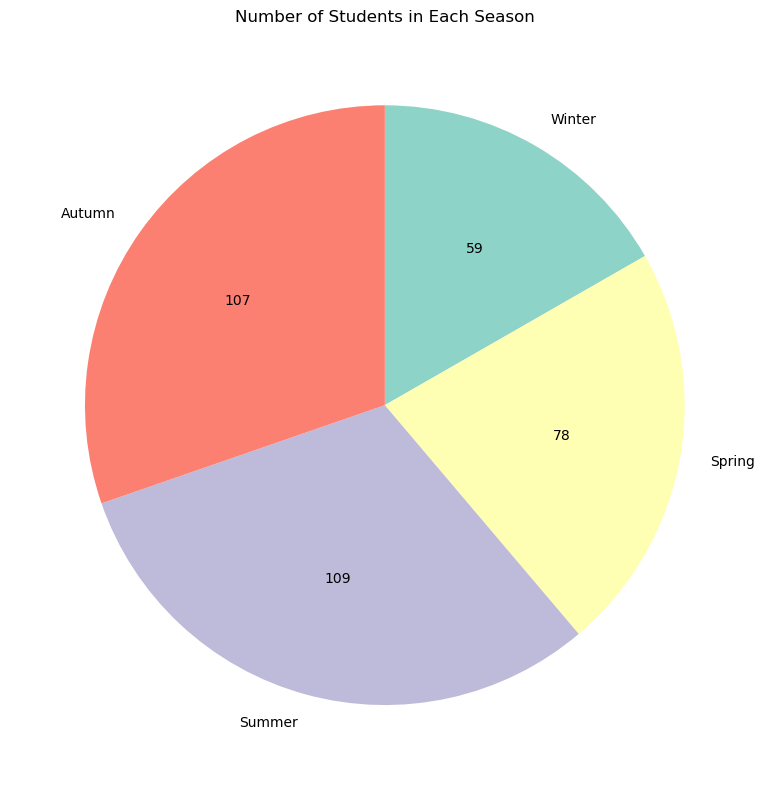
\includegraphics[width=0.6\textwidth]{Number of Students in Each Season (Pie Chart).png}
    \caption{Number of Students in Each Season}
    \label{fig:seasonal-students}
\end{figure}

\section*{3. Monthly Trend of Average Course Price}

The monthly trend of average course price is presented in Figure~\ref{fig:avg-course-price}. Barista and Sausage courses consistently have the highest average prices. Prices for some courses (e.g., Kabab, Pizza) increase in Autumn and Winter, possibly due to higher demand or pricing strategy changes. While not all course types are offered every month, the overall trend direction is still observable.

\begin{figure}[h!]
    \centering
    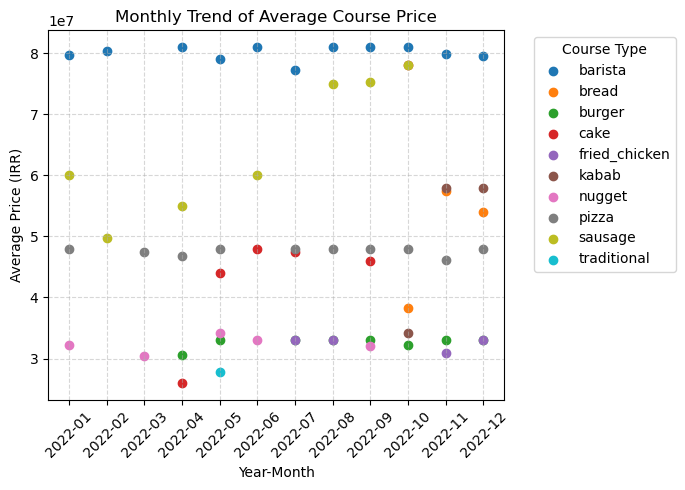
\includegraphics[width=0.76\textwidth]{Monthly Trend of Average Course Price.png}
    \caption{Monthly Trend of Average Course Price}
    \label{fig:avg-course-price}
\end{figure}

\section*{4. Distribution of Classes by Weekday}

As shown in Figure~\ref{fig:weekday-classes}, Thursday and Friday are the most common class days (each with 64 classes). Tuesday and Wednesday have the fewest classes, indicating a possible scheduling preference. This pattern suggests student availability or business strategy focuses on weekends.

\begin{figure}[h!]
    \centering
    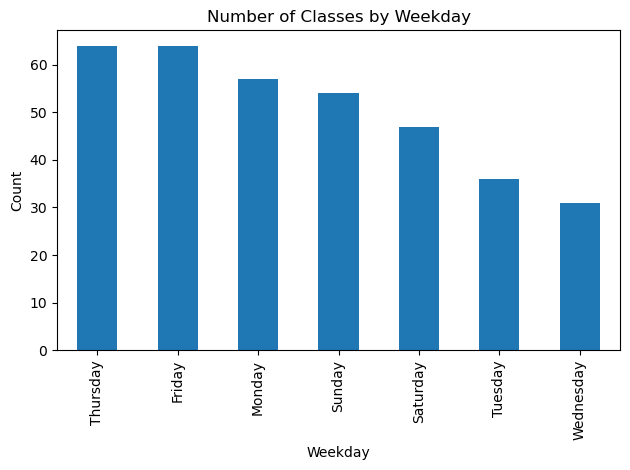
\includegraphics[width=0.7\textwidth]{Number of Classes by Weekday.png}
    \caption{Number of Classes by Weekday}
    \label{fig:weekday-classes}
\end{figure}

\section*{5. Calendar Heatmap of Class Days by Course Type}

Figure~\ref{fig:calendar-heatmap} presents the calendar heatmap of class days by course type. Class scheduling appears evenly distributed across the month. Certain course types (such as Barista and Burger) tend to be scheduled more often in the middle or towards the end of the month. This calendar view can support operational planning and spacing of similar courses.

\begin{figure}[h!]
    \centering
    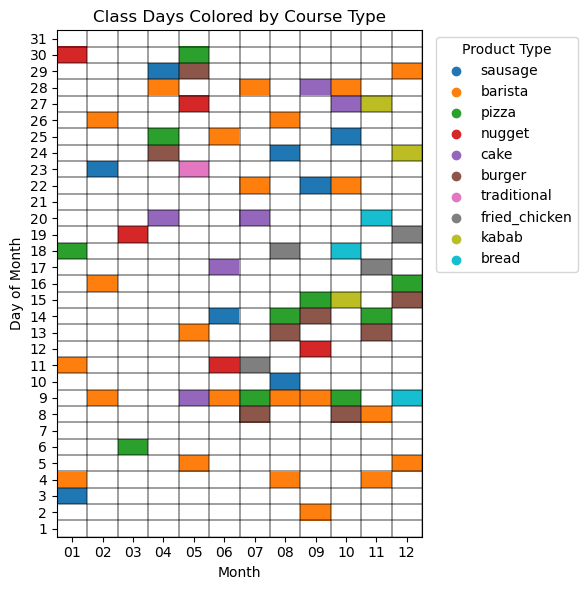
\includegraphics[width=1\textwidth]{Class Days Colored by Course Type.png}
    \caption{Calendar Heatmap of Class Days by Course Type}
    \label{fig:calendar-heatmap}
\end{figure}

\section*{Summary}

\begin{itemize}
    \item Summer and Autumn are peak seasons for student enrolment.
    \item Barista and Sausage courses dominate in pricing.
    \item Thursday and Friday are the most popular weekdays for classes.
    \item Course scheduling appears balanced, but with minor patterns based on course type.
\end{itemize}

\end{document}